\documentclass[10pt,a4paper]{article}
\usepackage[utf8]{inputenc}
\usepackage[english,russian]{babel}
\usepackage{cmap}
\usepackage[OT1]{fontenc}
\usepackage{amsmath}
\usepackage{amsfonts}
\usepackage{amssymb}
\usepackage{graphicx}
\usepackage{float}
\usepackage{wrapfig}
\usepackage{caption}
\DeclareCaptionLabelSeparator{dot}{. }
\captionsetup{justification=centering,labelsep=dot}
\graphicspath{{pictures/}}
\DeclareGraphicsExtensions{.pdf,.png,.jpg,.eps}
\begin{document}



\part{Планирование и управление}

\textbf{14	Марковские процессы принятия решений}\\

\textbf{14.1	Цели}

Это первая глава, посвящённая вероятностному \textit{планированию} и \textit{управлению} в книге. До сих пор предметом изложения было исключительно восприятие робота. Был описан широкий диапазон вероятностных алгоритмов для оценки интересующих параметров на основании данных датчиков. Однако, конечной целью работы любого программного обеспечения робота является выбор верных действий. В этой и следующих главах будут обсуждаться вероятностные алгоритмы по выбору действий.

Чтобы определить цели изучения вероятностных алгоритмов планирования, разберём следующие примеры.\\

1.	Манипулятор робота хватает и собирает части, прибывающие случайным образом по ленте конвейера. Конфигурация части в момент появления неизвестна, но стратегия оптимального манипулирования требует знания конфигурации. Как робот должен манипулировать такими частями? Будет ли необходимо восприятие? Если да, все ли методы восприятия одинаково хороши? Могут ли существовать стратегии манипулирования, дающие полностью определённую конфигурацию без восприятия?\\

2.	Подводный аппарат должен пройти от побережья Канады в Каспийское море. Должен ли он следовать кратчайшим маршрутом через Северный полюс, рискуя потерять ориентировку подо льдами? Или же необходимо следовать более длинным маршрутом по открытой воде, где возможна периодическая локализация с помощью GPS, глобальной космической системы позиционирования? До какой степени такие решения зависят от точности внутренних датчиков подводной лодки?\\

3.	Группа роботов исследует неизвестную планету с целью получения единой карты. Должны ли роботы искать друг друга, чтобы определить относительные местоположения? Или же им следует друг друга избегать, что позволит изучить больше новой территории за более короткое время? Как изменится оптимальная стратегия исследования, если относительные стартовые местоположения роботов неизвестны?\\

Эти примеры иллюстрируют, что выбор действия во многих задачах робототехники тесно связан с понятием неопределённости. В некоторых задачах, таких, как исследование с помощью роботов, уменьшение неопределённости является прямой целью, определяющей выбор действий.\\ 

ЗАДАЧА СБОРА ИНФОРМАЦИИ\\
Такие задачи известны как \textit{задачи сбора информации} и будут изучаться в Главе 17.
В других случаях уменьшение неопределённости имеет целью достижение какой-либо иной цели, например, обеспечения надёжности прибытия в целевое местоположение. Эти задачи будут изучены в этой и следующих главах.

С точки зрения разработки алгоритма, удобно выделить два типа неопределённости: неопределённость, вызванная действием и неопределённость восприятия.

Во-первых, отделим \textit{детерминированные} и стохастические эффекты действий. Многие теоретические результаты робототехники основаны на допущении, что эффекты действий управления детерминированы. Однако, на практике, действия порождают неопределённость, поскольку результат действий на самом деле не детерминирован. Неопределённость возникает в силу стохастической природы робота и его окружения, что требует восприятия параметров среды во время работы и возможности реагировать на неожиданные ситуации, даже если среда полностью наблюдаема. Недостаточно лишь запланировать единственную последовательность действий и слепо следовать ей.

Во-вторых, следует различать \textit{полностью наблюдаемые} и \textit{частично наблюдаемые системы}. В классической робототехнике часто считается, что датчики способны измерить полное состояние среды. Если бы это всегда было так, авторы бы не написали эту книгу! Фактически, ситуация строго противоположная. Практически во всех интересных задачах робототехники в реальном мире ограничения датчика являются ключевым фактором.

Очевидно, робот должен принимать во внимание текущую неопределённость, решая, что делать дальше. При выборе управляющего действия, как минимум, робот должен учитывать различные исходы (которые могут включать катастрофические отказы), взвешивая их согласно вероятностям того, что они действительно произойдут.\\

ОЖИДАЕМАЯ НЕОПРЕДЕЛЁННОСТЬ\\
Однако, управление роботом должно обрабатывать и будущую, \textit{ожидаемую неопределённость}. Пример приводился выше, при обсуждении робота, который может выбрать более короткий путь в среде без возможности пользоваться GPS, или же более длинный, но с меньшим риском потеряться. Уменьшение ожидаемой неопределённости важно во многих приложениях робототехники.

В ходе изложения будем придерживаться свободной точки зрения без разделения планирование и управления, поскольку, изначально, и планирование и управление преследуют единую цель – выбрать действия. 

Они отличаются в ограничениях времени, согласно которым следует выбирать действия, и роли восприятия при выполнении. Все алгоритмы, описанные в этой главе, схожи в том, что требует оффлайнового этапа оптимизации или планирования. Результатом этого этапа планирования является политика управления, предопределяющая действие управления для любой разумной ситуации. Другими словами, политика управления является эффективным контроллером, в том смысле, что ее можно использовать для определения действий робота с минимальным временем вычислений. Ни в коем случае выбор алгоритмов не предполагает, что это единственный способ обрабатывать неопределённость в робототехнике. Однако, он влияет на манеру использования алгоритмов, которые в настоящее время используются в области вероятностной робототехники.

В большей части алгоритмов, обсуждаемых в этой главе, подразумеваются конечные пространства состояний и действий. Непрерывные пространства аппроксимируются с помощью методов на основе сеток.

Следующие четыре главы организованы следующим образом.\\

•	В этой главе детально обсуждается роль двух типов неопределённости и закладываются основные шаблоны разработки алгоритмов. В качестве первого решения для ограниченного класса задач будет представлен  \textit{итерационный алгоритм}, популярное решение для вероятностных систем. Обсуждение в этой главе затронет только первый тип неопределённости: неопределённость в движении робота. Рассуждения основаны на допущении о том, что состояние полностью наблюдаемо. Лежащий в основе математический аппарат известен под названием \textit{марковские процессы принятия решений} (Markov decision processes - MDP).\\

•	В Главе 15 метод итерационного алгоритма обобщается для обоих типов неопределённости, эффектов движения и восприятия. В этом виде итерационный алгоритм применяется для выражения состояния в виде гипотезы. Математический аппарат в основе метода носит название "марковские процессы принятия решений с частичной наблюдаемостью" среды (partially observable Markov decision processes - POMDP). Алгоритмы POMDP обрабатывают неопределённость, активно собирая информацию, для достижения произвольной цели. В Главе 15 также обсуждаются различные эффективные аппроксимации, позволяющие лучше вычислять политики управления.\\

•	В Главе 16 вводятся некоторые итерационные алгоритмы для POMDP. Во всех решениях выполняется аппроксимация вероятностного процесса планирования для улучшения вычислительной эффективности. Один из таких алгоритмов позволит ускорить вероятностное планирование на основе допущения, что в какой-то момент в будущем состояние станет полностью наблюдаемым. Другой позволяет сжимать оценку состояния в представление с более низкой размерностью и выполняет планирование на основе этого представления. В третьем алгоритме для конденсации пространства задач используются многочастичные фильтры и методы машинного обучения. Все три этих алгоритма возможно существенно улучшить, уменьшив вычислительную сложность, хотя они уже достаточно применимы для практических задач робототехники.

\begin{figure}[H]
	\center{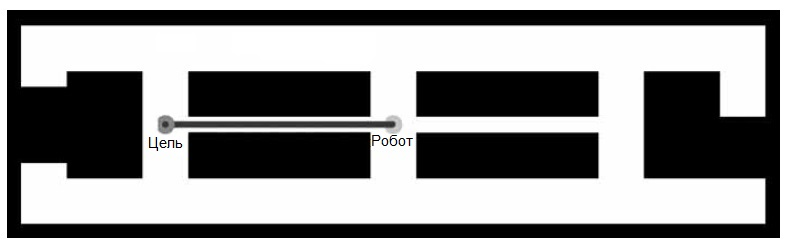
\includegraphics[width=0.9\linewidth]{141orig}}
	\caption{ ( Рис. 14.1 Почти симметричная среда с узкими и широкими коридорами. Робот начинает работу в центре с неизвестной ориентацией по направлению. Его целью является передвижение в пункт назначения слева.) }
	\label{fig:141orig}
\end{figure}

•	Глава 17 посвящена специализированной проблеме исследования с помощью роботов. Здесь задачей робота является сбор информации об окружающей среде. Хотя методы исследования касаются проблемы неопределённости датчика, задача существенно проще по сравнению с POMDP, а, значит, может быть решена более эффективно. Вероятностные методы исследования популярны в робототехнике, поскольку роботов часто используют для получения информации о неизвестных местах.\\

\textbf{14.2	Неопределённость в выборе действия}\\

На Рис. 14.1 показана упрощённая среда для иллюстрации различных типов неопределённости, с которой может столкнуться робот. На рисунке показан мобильный робот в среде, состоящей из коридоров. Среда обладает высокой степенью симметричности, и единственным различимым признаком является дальний конец коридора, имеющий разную форму в зависимости от места на карте. Робот начинает в указанном месте и ищет способ достичь целевого местоположения. Заметим, что до цели существует несколько путей, более короткий, но узкий, и два более длинных, но имеющих большую ширину.

В классической парадигме планирования с помощью роботов неопределённости нет. Робот просто знает своё начальное положение и местоположение цели. Более того, действия, выполненные в физическом мире, имеют прогнозируемые последствия, которые могут быть предварительно запланированы. В такой ситуации нет необходимости в восприятии.  Достаточно запланировать единственную последовательность действий, которая может выполняться в реальном времени. На Рис. 14.1 показан пример такого планирования. Очевидно, при отсутствии ошибок в движении робота, узкий путь предпочтительнее любого другого, более длинного пути. Поэтому «классический» планировщик всегда выберет первый, короткий путь.

\begin{figure}[H]
	\center{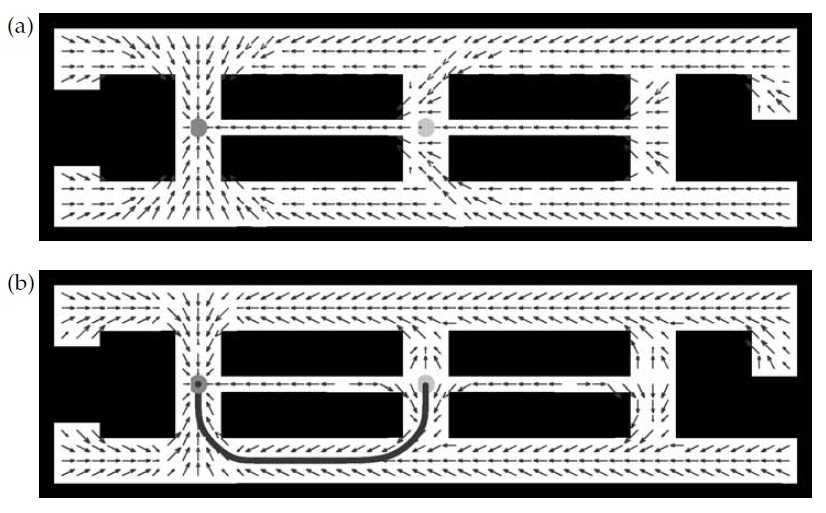
\includegraphics[width=0.9\linewidth]{142orig}}
	\caption{ ( Рис. 14.2 Функция подкрепления и политика управления в MDP с детерминированными (a) и недетерминированными эффектами действия (b). В детерминированной модели робот совершенно свободно выполняет навигацию по узкому пути. Длинный путь оказывается предпочтительнее, если результат действия не гарантирован, для предотвращения столкновения со стеной. На Рис. (b) показан такой путь.) }
	\label{fig:142orig}
\end{figure}

На практике такие планы не работают в силу нескольких причин. Робот, слепо следующий по узкому проходу, подвержен опасности столкновения со стеной. Более того, слепое выполнение команд может привести к промаху мимо целевого местоположения из-за ошибок при выполнении плана. Поэтому, на практике такие алгоритмы планирования часто комбинируются с реактивным модулем управления на основе датчиков, который подстраивает траекторию робота так, чтобы избежать столкновений. Такой модуль может предотвратить столкновение робота со стеной в узком коридоре, но для этого ему может понадобиться замедлить движение робота, что сделает длинный путь более предпочтительным.\\

МАРКОВСКИЙ ПРОЦЕСС ПРИНЯТИЯ РЕШЕНИЙ\\

Парадигма с учётом неопределённости движений робота известна как \textit{марковские процессы принятия решений} (Markov decision processes – MDP). В MDP предполагается, что состояние окружающей среды может полностью наблюдаться в любой момент времени. Другими словами, модель восприятия $p(z|x)$ детерминирована и взаимно однозначна. Однако, аппарат MDP позволяет учитывать и стохастические эффекты действия. Так, модель действия $p(x'u,x)$ может быть не детерминирована, а, следовательно, недостаточно просто запланировать одну последовательность действий. Вместо этого, планировщик должен генерировать действия для всего диапазона ситуаций, с которыми может столкнуться робот, в силу своих действий или непредсказуемой динамики окружающей среды. Одним из способов обработки результирующей неопределённости является генерация \textit{политики выбора действия}, определённая для всех состояний, в которых робот может оказаться.\\ 

ПОЛИТИКА УПРАВЛЕНИЯ\\
Такая проекция состояний в действия известна под многими названиями, например, \textit{политика управления}, \textit{универсальные планы}, и \textit{навигационные функции}. Пример политики показан на Рис. 14.2. Вместо единственной последовательности действий робот вычисляет проекции состояний в действия, показанные стрелками. После вычисления проекции робот способен обрабатывать отсутствие детерминированности восприятием состояния среды, и соответствующим образом реагировать. На Рис. 14.2a показана политика для робота с очень малой неопределённостью движения, когда проход по более узкому пути, действительно, допустим. На Рис. 14.2b показана та же ситуация, но для увеличившейся случайности в движениях робота. Здесь проход по узкому пути гораздо вероятнее приведёт к столкновению, и предпочтительным будет двигаться в обход. Этот пример иллюстрирует два факта: важность учёта неопределённости в процессе планирования движения, и возможность нахождения хорошей политики управления с помощью описанных алгоритмов.

\begin{figure}[H]
	\center{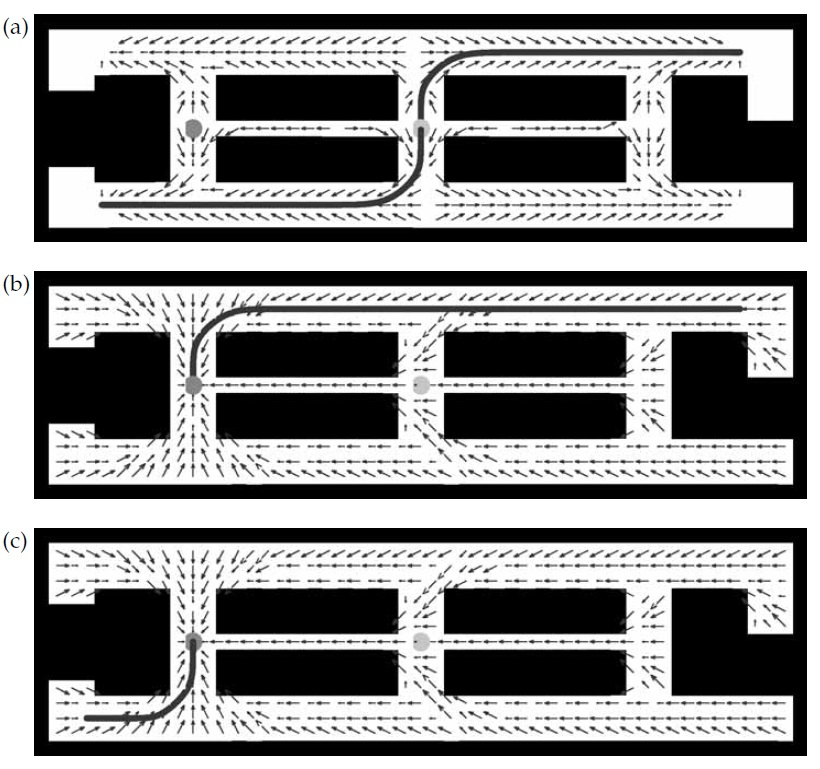
\includegraphics[width=0.9\linewidth]{143orig}}
	\caption{ ( Рис. 14.3 Сбор информации в POMDP: Для достижения цели с более чем 50\% вероятностью, планировщик в пространстве оценок сначала выполняет навигацию до местоположения, глобальную ориентацию которого можно определить. На Рис. (a) показана политика соответствия и возможный путь следования робота. На основании текущего местоположения робот может обнаружить, что находится в точке (b) или (c), из которой можно безопасно передвигаться к цели.) }
	\label{fig:143orig}
\end{figure}

МАРКОВСКИЕ ПРОЦЕССЫ ПРИНЯТИЯ РЕШЕНИЙ С ЧАСТИЧНОЙ НАБЛЮДАЕМОСТЬЮ СРЕДЫ\\

Вернёмся к более общему, полностью вероятностному случаю, отбросив допущение о полной наблюдаемости состояния. Этот случай известен как \textit{марковские процессы принятия решений с частичной наблюдаемостью среды} (partially observable Markov decision processes – POMDP). Во многих, если не во всех, робототехнических реализациях, измерения $z$ являются зашумлёнными проекциями состояния $x$. В силу этого, состояние можно оценить лишь до некоторой степени. Проиллюстрируем это с помощью уже приведённого примера, но с другими допущениями. Допустим, робот осведомлен о своей начальной позиции, но не знает, ориентирован ли по направлению налево, или направо. Более того, датчика, способного определить прибытие к цели, у него нет.

Конечно, симметрия среды сильно затрудняет определение верной ориентации. Двигаясь напрямую к проекции цели впереди, робот имеет 50\% шанс промахнуться мимо цели, придя в симметричное местоположение в правой части среды. Поэтому, оптимальный план – двигаться к любому из углов среды, где признаков уже будет достаточно для определения ориентации. Политика передвижения в эти местоположения показана на Рис. 14.3a. Основываясь на начальной ориентации по направлению, робот может передвинуться по любому из двух показанных путей. При достижении угла его датчики определяют ориентацию по направлению, получая текущее местоположение относительно среды. Робот может обнаружить, что находится в одной из двух ситуаций, показанных на Рис 14.3b и c, откуда он может безопасно переместиться к цели.

На этом примере показан один из ключевых аспектов вероятностной робототехники. Роботу необходимо активно собирать информацию, и, чтобы это сделать, приходится идти в обход, что не является важным для робота, воспринимающего своё положение с абсолютной точностью. Это проблема очень важна в робототехнике. Почти для всех задач робототехники датчики робота характеризуются изначальными ограничениями того, что робот способен узнать, и где может быть получена информация. Похожие ситуации встречаются в задачах вида «обнаружить и вернуть», планетарных исследованиях, поиске и спасении в городе и так далее.

Возникает вопрос, каким же образом вывести алгоритм для выбора действий, способный работать с таким типом неопределённости. Как мы узнаем, вопрос далеко не тривиальный. На первый взгляд, кажется продуктивным проанализировать каждую ситуацию, возможную при текущем уровне осведомлённости. В нашем примере таких ситуаций две. В первом случае цель находится сверху слева относительно начального положения робота, а во втором – снизу справа. В обоих случаях, однако, оптимальной политикой является не перемещение агента к цели, а увод его к точке, где он будет способен разрешить двойственность восприятия своего положения. Поэтому, задача планирования в частично наблюдаемой среде не может быть решена с помощью учёта всех возможных сред и усреднения решения.

Вместо этого, базовой идеей будет генерация планов в \textit{пространстве гипотез}, синоним термина \textit{информационное пространство}. Пространство гипотез состоит из пространства всех апостериорных гипотез о состоянии окружающего мира, которые могут быть у робота. Пространство гипотез в нашем простом примере соответствует трём врезкам на Рис. 14.3. На верхней врезке показан пример гипотезы в пространстве гипотез. На ней показана начальная политика, когда робот не осведомлен о своём положении в пространстве. Согласно этой политике, робот перемещается к одному из углов среды, где он в состоянии выполнить локализацию. После локализации он может безопасно следовать далее к цели, как показано на двух нижних врезках Рис. 14.3. Поскольку априорный шанс каждой ориентации в пространстве одинаковый, робот будет перемещаться, имея 50\% шансы оказаться в одном из двух положений, показанных ниже.

В нашем упрощённом примере, количество разных оценок состояний конечно: робот точно знает своё местоположение или же не имеет о нем ни малейшего понятия. В практических реализациях это обычно не так. В средах с конечным множеством состояний пространство гипотез обычно непрерывно, но имеет конечную размерность. Фактически, количество измерений пространства гипотез имеет тот же порядок, что и количество состояний в подлежащем пространстве состояний. Если пространство состояний непрерывно, пространство гипотез имеет бесконечно много измерений.

Этот пример иллюстрирует фундаментальное свойство, возникающее из невозможности идеального восприятия состояния среды роботом, важность которого в робототехнике так часто недооценивают. В неопределённых средах алгоритм планирования робота должен учитывать состояние осведомлённости в принятии решений управления. В общем случае, недостаточно учитывать только самое вероятное состояние. Устанавливая зависимость движения от гипотезы состояния, в отличие от наиболее вероятного состояния, робот может активно выполнять сбор информации. Фактически, оптимальный план для гипотезы состояния предусматривает «оптимальный» сбор информации, поскольку ищет только новую информацию и лишь в той степени, которая будет полезна для возможного использования в действиях робота. Возможность получения оптимальных политик управления является ключевым преимуществом вероятностного подхода в робототехнике по сравнению с классическим детерминированным, «всеведающим» подходом. Однако, как скоро будет показано, за него приходится платить цену в виде возросшей сложности задачи планирования.\\

\textbf{14.3	Итерационный алгоритм}\\

Первый алгоритм для нахождения политик управления называется \textit{итерационный алгоритм}. итерационный алгоритм рекурсивно выполняет вычисление полезности каждого действия относительно функции подкрепления. Обсуждение в этой главе будет ограничено первым типом неопределённости – стохастичностью робота и физического мира. Отложим до следующей главы рассмотрение неопределённости, возникающее из ограничений датчика. Пока что будем считать, что состояние среды полностью наблюдаемо в произвольный момент времени.\\

\textbf{14.3.1	Цели и подкрепление}

Перед описанием конкретного алгоритма, определим задачу в более точных терминах.\\ 
ЦЕЛЬ\\
В общем случае, выбор действий робота обусловлен \textit{целями}. Цели могут соответствовать определенным конфигурациям (например, часть была успешно подобрана и размещена манипулятором робота), выражена условиями в течение длительного времени (робот сохраняет баланс шеста).\\

СТОИМОСТЬ\\
В робототехнике иногда необходимо достичь некой целевой конфигурации, одновременно оптимизируя другие переменные, часто воспринимаемые как \textit{стоимость}. Например, целью может быть перемещение конечного эффектора манипулятора в конкретное местоположение, одновременно минимизируя время, потребление энергии или количество столкновений с препятствиями. 

На первый взгляд, может показаться затруднительным выражение этих условий двумя параметрами, один из которых максимизируется (например, бинарный флаг, показывающий, достиг ли робот целевого местоположения), а вторая – сводится к минимуму (например, общее энергопотребление робота).\\ 

ФУНКЦИЯ ПОДКРЕПЛЕНИЯ\\
Однако, обе можно выразить с помощью одной функции, которая называется \textit{функция подкрепления}.

Доход, обозначаемый $r$, является функцией состояния и управления роботом. Например, простая функция подкрепления может иметь следующий вид:\\

(14.1)
\begin{equation*}
r(x,u)= \left\{
\begin{array}{ll}
+100& \mbox{если \textit{u} ведет к целевой конфигурации или состоянию}\\
-1& \mbox{во всех остальных случаях}
\end{array}
\right.
\end{equation*}

Эта функция «награждает» робота +100 при достижении целевой конфигурации, и «штрафует» робота -1 на каждый такт времени, когда он не достиг искомой конфигурации. Такая функция подкрепления даст максимальный суммарный доход, если робот достигает целевой конфигурации за минимально возможное время.

Зачем использовать одну переменную награды для выражения достижения цели и стоимости? Главным образом, причин две. Во-первых, такая нотация позволяет избежать беспорядка в следующих формулах, поскольку должна объединять обработку стоимости и достижения цели в целях изложения в книге. Во-вторых, что более важно, в ней отдаётся должное фундаментальному компромиссу между достижением цели и стоимости прохода по пути. Поскольку роботы изначально неопределены, нет возможности определить была ли достигнута целевая конфигурация. Вместо этого, все, на что можно надеяться, это максимизация шансов достижения цели. Этот компромисс между достижением цели и стоимостью характеризуется такими вопросами, как \textit{стоит ли увеличение вероятности достижения цели дополнительных усилий (например, в смысле времени или энергии)?} Считая достижение цели и стоимость одним числовым множителем позволяет разменивать и настраивать переменные, давая целостный способ выбора действий в условиях неопределённости.

Наша задача – вывести программу генерации действий таким образом, чтобы оптимизировать будущие ожидаемые затраты.\\

ПОЛИТИКА\\
Такую программу обычно называют \textit{политикой управления}, или, проще, \textit{политикой}. Обозначим ее следующим образом:\\

(14.2)
$$\pi:z_{1:t-1},u_{1:t-1}\longrightarrow u_t$$

В случае полной наблюдаемости среды, допустим намного более простой случай:\\

(14.3)
$$\pi:x_r\longrightarrow u_t$$

Таким образом, $\pi$ является функцией, которая проектирует прошлые данные в управляющие воздействия или же состояния в управляющие воздействия, когда состояние наблюдаемо.

Пока что, в нашем определении политики управления не было сделано никаких утверждений относительно вычислительных свойств. Это должен быть быстрый реактивный алгоритм, полагающийся на решения на основе самого последнего  элемента, или же тщательно подобранный алгоритм планирования. На практике, однако, вычислительные соображения важны, поскольку любая задержка вычисления управляющего воздействия может негативно повлиять на работу робота. Определение политики $\pi$ также не даёт никакого утверждение относительно ее детерминированности.\\

ГОРИЗОНТ ПЛАНИРОВАНИЯ\\

Интересной концепцией в контексте создания политик управления является \textit{горизонт планирования}. Иногда достаточно выбрать управляющее действие таким образом, чтобы максимизировать следующее значение награды. В большинстве случаев действие не приведёт к немедленной награде. Например, робот, который перемещается к целевому местоположению, получит финальную награду при достижении цели только после самого последнего действия. Очевидно, что награда может быть отсрочена.\\ 
СУММАРНЫЙ ДОХОД\\
Тогда подходящей целью будет выбор таких действий, которые бы привели к максимальной сумме итогового дохода. Назовём эту сумму \textit{суммарным доходом}. Поскольку мир не детерминирован, лучше всего оптимизировать \textit{ожидаемый суммарный доход}, которую удобно записать в виде\\

(14.4)
$$R_T=E\left[\sum_{r=1}^T \gamma^Tr_{t+\tau} \right] $$

Здесь ожидание $E[ ]$ берётся по моментальным значениям будущего дохода $r_{t+\tau}$ который робот может получить между моментами времени $t+T$.\\ 
КОЭФФИЦИЕНТ ПЕРЕОЦЕНКИ\\
Отдельные значения дохода $r_{t+\tau}$ умножаются на множитель $\gamma^T$, называемым \textit{коэффициент переоценки}. Значение $\gamma$ является параметром, специфичным для задачи, и ограничивается интервалом $[0; 1]$. Если $\gamma = 1$, получим $\gamma^T = 1$ для произвольных значений $\tau$,  а, значит, в выражении (14.4) можно опустить множитель. Меньшие значения $\gamma$ экспоненциально уменьшают будущий доход, делая раннее получение награды экспоненциально более важным. Этот коэффициент переоценки, важность которого будет обсуждаться позже, напоминает концепцию денег, которые теряют стоимость экспоненциально по времени из-за инфляции.

ГОРИЗОНТ ПЛАНИРОВАНИЯ\\

Заметим, что $R_T$ является суммой $T$ тактов времени. $T$ называется \textit{горизонтом планирования}, или, проще, \textit{горизонтом}. Будем различать три важных случая:\\

ЖАДНЫЙ СЛУЧАЙ\\

1.	$T = 1$. Ситуация, когда робот стремится  минимизировать следующий штраф, называется \textit{жадным случаем}. Хотя случай вырожденный и эффект действий, кроме как на следующем такте времени, не рассматриваются, на практике он довольно важен, поскольку жадная оптимизация проста по сравнению с оптимизацией для нескольких тактов. Во многих задачах робототехники жадные алгоритмы являются лучшими на сегодняшний день решениями, которые могут быть вычислены за полиномиальное время. Очевидно, жадная оптимизация инвариантна по отношению к коэффициенту скидки $\gamma$, но требует, чтобы $\gamma>0$.\\

СЛУЧАЙ КОНЕЧНОГО ГОРИЗОНТА\\

2.	T больше 1, но конечно. Этот случай известен как \textit{случай конечного горизонта}. Обычно, доход не падает со временем, поэтому $\gamma = 1$. Можно аргументировать, что случай конечного горизонта единственный, который имеет значение, поскольку во всех практических задачах время конечно. Однако, оптимальность конечного горизонта часто труднее достичь, чем оптимальность в случае бесконечного горизонта с переоценкой. Почему это так? Во-первых, заметим, что оптимальное управляющее действие является функцией временного горизонта. Например, около дальнего конца временного горизонта оптимальная политика может существенно отличаться от оптимального выбора в более ранний момент времени, даже при прочих одинаковых условиях (то же состояние и тот же прогноз). В результате, алгоритмы планирования с конечным горизонтом должны сохранять разные пути для разных горизонтов, что добавляет нежелательную сложность.\\

СЛУЧАЙ С БЕСКОНЕЧНЫМ ГОРИЗОНТОМ\\

3.	$T$ бесконечно. Этот случай известен как \textit{случай с бесконечным горизонтом}. Он не подвержен проблемам, применимым для случая с конечным горизонтом, поскольку количество оставшихся шагов времени в любой мент времени одинаково (и бесконечно!). Однако, присутствие коэффициента переоценки $\gamma$ крайне важно. Чтобы понять почему, давайте разберём случай, когда имеются две программы управления роботом, одна, зарабатывающая \$1 в час, и вторая, зарабатывающая \$100 в час. В случае конечного горизонта, вторая программа, очевидно, предпочтительнее первой. Неважно, каково значение горизонта, ожидаемая накопленная награда превышает награду первой программы в сто раз. Для случая бесконечного горизонта это не так. Без переоценки обе программы заработаю бесконечно много денег, что делает ожидаемый суммарный доход $R_T$ несущественным при выборе программы.\\

При допущении, что каждая отдельная награда $r$ ограничена по размеру (так, чтобы, $|r|<r_{\max}$ для некоторого $r_{\max}$), переоценка гарантирует, что $R_\infty$ конечно, несмотря на факт того, что сумма состоит из бесконечного множества слагаемых. А именно, получим\\

(14.5)
$$R_\infty\leq r_{\max}+\gamma r_{\max}+\gamma^2r_{\max}+\gamma^3r_{\max}+...=\frac{r_{\max}}{1-\gamma}$$

Это показывает, что $R_\infty$ конечно до тех пор, пока $\gamma$ меньше 1. Попутно заметим, что альтернатива переоценке включает максимизацию среднего дохода, вместо полного. Алгоритмы максимизации среднего дохода не будут рассматриваться в книге.\\

Иногда будем обращаться к суммарному доходу $R_T$, который  зависит от состояния $x_t$. Это можно записать в следующем виде:\\

(14.6)
$$R_T(x_t)=E\left[\sum_{\tau=1}^T \gamma^Tr_{t+\tau}|x_t\right]$$ 

суммарный доход $R_T$ является функцией политики выбора действий робота. Иногда выгодно сделать эту зависимость явной:\\

(14.7)
$$R_T^\pi(x_t)=E\left[\sum_{\tau=1}^T \gamma^Tr_{t+\tau}|u_{t+\tau}=\pi(z_{1:t+\tau-1},u_{1:t+\tau-1})\right]$$

Такая запись позволяет сравнить две политики управления $\pi$ и $\pi'$, и определить, какая лучше. Просто сравним $R_T^\pi$ и $R_T^{\pi'}$  и выберем алгоритм с более высоким ожидаемым будущим доходом с учётом переоценки!\\

\textbf{14.3.2	Нахождение оптимальных политик управления для случая полной наблюдаемости}\\

Эту главу необходимо завершить алгоритмом итерации значений для вычисления политик управления в полностью наблюдаемых средах. На первый взгляд, такие алгоритмы отходят от общих допущений вероятностной робототехники, в частности о том, что состояние ненаблюдаемо. Однако, в некоторых реализациях вполне допустимо считать, что апостериорная вероятность $p(x_t|z_{1:t}, u_{1:t})$ хорошо выражается математическим ожиданием $E[p(x_t|z_{1:t}, u_{1:t})]$.

Случай полной наблюдаемости имеет ряд достоинств. Обсуждаемый алгоритм также подготовит почву для более общего случая частичной наблюдаемости.

Также заметим, что способы отображения стохастических сред с полностью наблюдаемым состоянием известны как марковские процессы принятия решений. Политики в MDP являются проекциями состояния на управляющие действия:\\

(14.8)
$$\pi:x\longrightarrow u$$

Факт того, что состояния достаточно для определения оптимального управления является прямым следствием марковского свойства, которое подробно обсуждалось в подразделе 2.4.4. Целью планирования в терминах MDP является обнаружение такой политики $\pi$, которая максимизирует будущий суммарный доход.

Начнём с определения оптимальной политики для горизонта планирования $T = 1$, поскольку нас интересует только политика, максимизирующая следующую награду. Эта политика должна обозначаться $\pi_1(x)$ и получаться путём максимизации ожидаемого дохода за один шаг по всем управляющим действиям:\\

(14.9)
$$\pi_1(x)=\underset{u}{\text{argmax}}\,r(x,u)$$

Оптимальным действием будет то, которое то, которое обеспечит максимальный ожидаемый доход, который возможно получить немедленно. Политика, выбирающая такое действие, оптимальна по ожиданию. 

ФУНКЦИЯ ДОХОДОВ\\

Для каждой политики есть связанная  функция доходов, измеряющая ожидаемое значение (суммарный будущий доход со с переоценкой). Для $\pi_1$, функция доходов, это просто ожидаемая немедленная награда, уменьшенная коэффициентом переоценки $\gamma$:\\

(14.10)
$$V_1(x)=\gamma\,\underset{u}{\max}\,r(x,u)$$

Это значение для более дальних горизонтов планирования теперь определяется рекурсивно. Оптимальная политика для горизонта $T = 2$ выберет управляющее действие, которое максимизирует сумму дохода на одном шаге $V_1(x)$ и немедленную награду на одном шаге:\\

(14.11)
$$\pi_2(x)=\underset{u}{\text{argmax}}\,\left[r(x,u)+\int V_1(x')\,p(x'|u,x)dx'\right]$$ 

Должно быть ясно, почему эта политика оптимальна. Значение этой политики зависит от состояния $x$, заданного следующим выражением с учётом переоценки:

(14.12)
$$V_2(x)=\gamma\,\underset{u}{\text{max}}\,\left[r(x,u)+\int V_1(x')\,p(x'|u,x)dx'\right]$$

Оптимальная политика и ее функция дохода для $T = 2$ была рекурсивно построена из оптимальной функции дохода для $T = 1$. Это наблюдение подразумевает, что для любого конечного горизонта $T$ оптимальная политика и связанная с ней функция дохода, может быть получена рекурсивно из оптимальной политики и функции дохода для $T-1$.

(14.13)
$$\pi_T(x)=\underset{u}{\text{argmax}}\,\left[r(x,u)+\int V_{T-1}(x')\,p(x'|u,x)dx'\right]$$

Результирующая политика $\pi_T (x)$ оптимальна для горизонта планирования $T$. Связанная функция дохода определена через следующую рекурсию:\\

(14.14)
$$V_T(x)=\gamma\,\underset{u}{\text{max}}\,\left[r(x,u)+\int V_{T-1}(x')\,p(x'|u,x)dx'\right]$$

В случае бесконечного горизонта, оптимальная функция дохода стремится к достижению равновесия (за исключением редких детерминированных систем, где такого равновесия не существует):\\

(14.15)
$$V_\infty(x)=\gamma\,\underset{u}{\text{max}}\,\left[r(x,u)+\int V_\infty(x')\,p(x'|u,x)dx'\right]$$

УРАВНЕНИЕ БЕЛЛМАНА\\

Эта инвариативность известна как \textit{уравнение Беллмана}. Без приведения доказательства заметим, что для каждой функции дохода $V$, условие (14.15) необходимо и достаточно, чтобы получившаяся политика была \textit{оптимальной}.\\

\textbf{14.3.3	Вычисление функции дохода}\\

Указанное соображение позволяет получить практический алгоритм вычисления оптимальной политики в стохастических системах с полностью наблюдаемым состоянием. Итерационный алгоритм выполняется путём последовательной аппроксимации функций оптимального дохода, как определено в (14.15).

Более детально, обозначим аппроксимацию функции дохода через $\hat{V}$. Изначально, $\hat{V}$ установлено в $r_{\min}$, минимально возможный немедленный доход:\\

(14.16)
$$\hat{V}\longleftarrow r_{\min}$$

Итерационный алгоритм затем последовательно обновляет аппроксимацию на основании следующего рекурсивного правила вычисления функции дохода для возрастающих горизонтов:\\

(14.17) 
$$\hat{V}(x)\longleftarrow\gamma\,\underset{u}{\text{max}}\left[r(x,u)+\int \hat{V}_(x')\,p(x'|u,x)dx' \right]$$

ОБРАТНЫЙ МЕТОД ПРоГОНКИ\\

Поскольку при каждом обновлении информация распространяется в обратном временном порядке через функцию ценности, это обычно называется \textit{обратный метод прогонки}.

Итерационный алгоритм имеет сильное сходство с приведённым выше вычислением оптимальной политики для $T$-горизонта. Итерационный алгоритм сходится при $\gamma<1$, а в некоторых особых случаях, даже при $\gamma = 1$. Порядок обновления состояний неважен до тех пор, пока каждое состояние обновляется бесконечно часто. На практике, сходимость обычно наблюдается после небольшого числа итераций.

В произвольный момент времени функция дохода $\hat{V}(x)$ определяет политику:\\

(14.18)
$$\pi(x)=\underset{u}{\text{argmax}}\,\left[r(x,u)+\int \hat{V}(x')\,p(x'|u,x)dx'\right]$$

После сходимости итерации ценности, жадная политика по отношению к конечной функции дохода является оптимальной.

Заметим, что все эти уравнения были сформулированы для общих пространств состояний. Для конечных пространств состояний, интеграл в каждом уравнении можно представить в виде конечной суммы по всем состояниям. Эту сумму часто можно эффективно вычислить, поскольку $p(x'|u, x)$ будет ненулевым для относительно небольшого количества состояний $x$ и $x'$. Это приводит к эффективному семейству алгоритмов вычисления функций дохода.

В Таблице 14.1 показаны три алгоритма: общий Итерационный алгоритм \textbf{MDP\_value\_iteration} для произвольных пространств состояний и действий, его дискретный вариант для конечных пространств состояний \textbf{MDP\_discrete\_value\_iteration}, и алгоритм получения оптимального управляющего действия из функции дохода, \textbf{policy\_MDP}. 

\begin{table}[H]
\begin{center}
\begin{tabular}{|l|}
\hline
{}\\
1:\textbf{ Algorithm MDP\_value\_iteration}$():\qquad\qquad\quad\qquad\qquad$\\
2:\hspace{5mm}$\textit{для всех}\,x\,\textit{do}$\\
3:\hspace{10mm}$\hat{V}(x)=r_{\min}$\\
4:\hspace{5mm}$\textit{endfor}$\\
5:\hspace{5mm}$\textit{повторять до сходимости}$\\
6:\hspace{10mm}$\textit{для всех}\,x$\\
7:\hspace{15mm}$\hat{V}(x)=\gamma\,\underset{u}{\text{max}}\left[r(x,u)+\int \hat{V}(x')\,p(x'|u,x)dx' \right]$\\
8:\hspace{10mm}$\textit{endfor}$\\
9:\hspace{5mm}$\textit{endrepeat}$\\
10:\hspace{5mm}$\textit{return}\,\,\hat{V}$\\
{}\\
\hline
\end{tabular}
\end{center}
\end{table}

\begin{table}[H]
\begin{center}
\begin{tabular}{|l|}
\hline
{}\\
1:\textbf{ Algorithm MDP\_discrete\_value\_iteration}$():\qquad\quad\qquad\qquad$\\
2:\hspace{5mm}$\textit{for}\,i=1\,\textit{to}\,N\,\textit{do}$\\
3:\hspace{10mm}$\hat{V}(x_t)=r_{\min}$\\
4:\hspace{5mm}$\textit{endfor}$\\
5:\hspace{5mm}$\textit{повторять до сходимости}$\\
6:\hspace{10mm}$\textit{for}\,i=1\,\textit{to}\,N\,\textit{do}$\\
7:\hspace{15mm}$\hat{V}(x_t)=\gamma\,\underset{u}{\text{max}}\left[r(x_t,u)+\sum_{j=1}^N \hat{V}(x_j)\,p(x_j|u,x_i) \right]$\\
8:\hspace{10mm}$\textit{endfor}$\\
9:\hspace{5mm}$\textit{endrepeat}$\\
10:\hspace{5mm}$\textit{return}\,\,\hat{V}$\\
{}\\
\hline
\end{tabular}
\end{center}
\end{table}

\begin{table}[H]
\begin{center}
\begin{tabular}{|l|}
\hline
{}\\
1:\textbf{ Algorithm policy\_MDP}$(x,\hat{V}):\qquad\quad\qquad\qquad\qquad\qquad\qquad$\\
2:\hspace{5mm}$\textit{return}\,\,\,\underset{u}{\text{argmax}}\left[r(x,u)+\sum_{j=1}^N \hat{V}(x_j)\,p(x_j|u,x_i) \right]$\\
{}\\
\hline
\end{tabular}
\caption{(Таблица 14.1 Итерационный алгоритм для MDP с конечными пространствами состояний и управляющих действий, показан в самом общем виде. Нижний алгоритм вычисляет наилучшее действие управления. )}
\end{center}
\end{table}			
\begin{figure}[H]
	\center{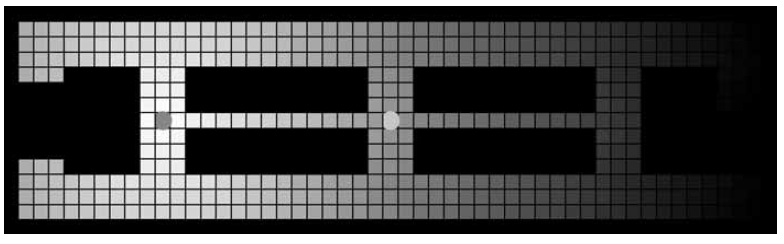
\includegraphics[width=0.9\linewidth]{144orig}}
	\caption{ ( Рис. 14.4 Пример функции дохода с бесконечным горизонтом $T_\infty$, подразумевая, что целевым состоянием является «поглощающее состояние». Эта функция дохода порождает политику, показанную на Рис. 14.2a.) }
	\label{fig:144orig}
\end{figure}			
Первый алгоритм \textbf{MDP\_value\_iteration} инициализирует функцию дохода в строке 3. В строках с 5 по 9 выполняются рекурсивные вычисления функции дохода. После сходимости итерационного алгоритма, результирующая функция дохода $\hat{V}$ порождает оптимальную политику. Если пространство состояний конечно, интеграл заменяется коечной суммой, как показано в \textbf{MDP\_discrete\_value\_iteration}. Множитель $\gamma$ является коэффициентом переоценки. Алгоритм \textbf{policy\_MDP} обрабатывает функцию оптимального дохода по состоянию $x$, и возвращает управляющее воздействие $u$, которая максимизирует ожидаемый доход.			
На Рис. 14.4 показан пример функции дохода для обсуждаемого выше примера. Здесь заливка ячеек сети соответствует их значению, значение, отмеченное белым $V = 100$, чёрным $V = 0$. Функция поиска экстремума в функции дохода основана на выражении 14.18, и ведёт к политике, показанной на Рис. 14.2a.\\			
			
\textbf{14.4	Применение к управлению роботом}\\

Простой итерационный алгоритм применим для задач с низкой размерностью управления и планирования движения робота. Для решения введём две аппроксимации.			
Во-первых, алгоритм в Таблице 14.5 определяет функцию дохода и требует максимизации и интеграции в непрерывном пространстве. На практике, принято аппроксимировать пространство состояний дискретным разложением, близким к гистограммированию, описанному в Главе 4.1. Похожим образом, дискретизируется пространство управляющих воздействий. Функция $\hat{V}$ легко реализуется в виде таблицы поиска, но такая декомпозиция работает только для пространств состояния и управления с низкой размерностью, в силу подверженности  "проклятью размерности". В ситуациях с большей размерностью для представления функции ценности вводятся обучающиеся алгоритмы.	
	
\begin{figure}[H]
	\center{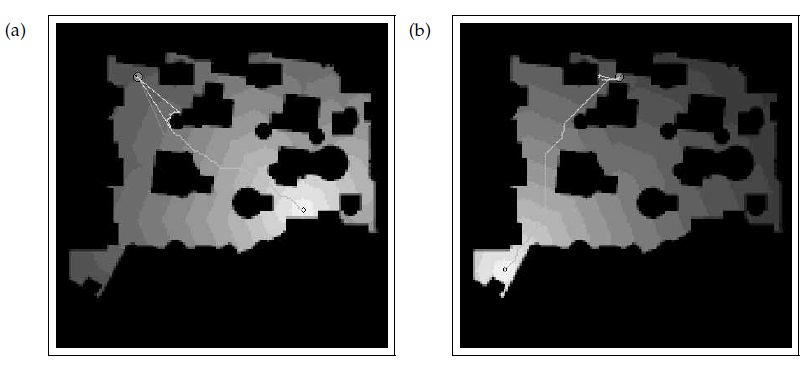
\includegraphics[width=0.9\linewidth]{145orig}}
	\caption{ ( Рис. 14.5 Пример итерационного алгоритма в пространстве состояний при движении робота. Препятствия показаны чёрным. Функция дохода обозначена серой заливкой. Жадный выбор действия по отношению к функции дохода позволяет найти оптимальный сигнал управления, считая, что положение робота наблюдаемо. Также на схемах показаны примерные пути, полученные в результате следования жадной политике.) }
	\label{fig:145orig}
\end{figure}	
	
Во-вторых, необходимо знать состояние! Как уже обсуждалось выше, может оказаться выигрышной замена апостериорного распределения его модой\\

(14.19)	
$$\hat{x}_t=E[p(x_t|z_{1:t},u_{1:t})]$$	
	
В контексте локализации робота такая аппроксимация работает хорошо, если мы сможем гарантировать, что робот всегда приблизительно локализован, а оставшаяся неопределённость апостериорного распределения локальна. Такой подход не работает, когда робот выполняет глобальную локализацию, или же был "похищен".	
	
На Рис. 14.5 показана итерация ценности в контексте задачи планирования пути робота. Здесь показана двухмерная проекция пространства конфигурации круглого робота. Пространство конфигураций – это пространство всех координат $(x, y, \theta)$ в которых робот может физически оказаться. Для круглых роботов пространство конфигурации получается «выращиванием» препятствий на карте основываясь на величине радиуса робота. Эти возвышающиеся препятствия показаны чёрным на Рис. 14.5.

Функция дохода показана градациями серого цвета, и чем светлее местоположение, тем выше её значение. Путь получен следованием оптимальной политике до соответствующего местоположения цели, как показано на Рис. 14.5. Из рисунка видно, что функция дохода определена по всему пространству состояний, и это позволяет роботу определять требуемое действие вне зависимости от своего положения. Это важно для недетерминированных сред, где действия стохастически влияют на состояние робота.

\begin{figure}[H]
	\center{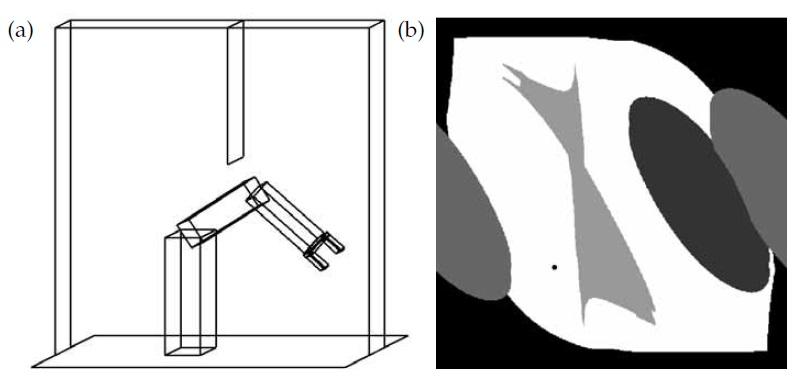
\includegraphics[width=0.9\linewidth]{146orig}}
	\caption{ ( Рис. 14.6 (a) 2-DOF манипулятор робота в пространстве с препятствиями. (b) \textit{Пространство конфигураций} этого манипулятора: горизонтальная ось соответствует плечевому сочленению, а вертикальная – конфигурации локтевого сочленения. Препятствия показаны серым. Маленькая точка на схеме соответствует конфигурации, показанной слева) }
	\label{fig:146orig}
\end{figure}

В планировщике пути, с помощью которого был сгенерирован Рис. 14.5, приняты особые допущения для поддержания приемлемой вычислительной нагрузки. Для круглых роботов, способных повернуться на одном месте, часто используется вычисление функции ценности только в плоских евклидовых координатах, игнорируя затраты на вращение. Также игнорируются переменные состояния, такие, как скорость робота, несмотря на то, что величина скорости очевидным образом ограничивает места, куда робот может переместиться в заданный момент времени. Для превращения политики управления в реальные команды общепринятой практикой является комбинирование таких планировщиков пути с быстрыми, реактивными модулями предотвращения столкновений, способными генерировать требуемые значения скорости вращения двигателей при соблюдении динамических ограничений. Планировщик пути, учитывающий полное состояние робота, может действовать, минимум, в пяти измерениях, состоящих из полного положения (три измерения), поступательной и вращательной скоростей робота. В двух измерениях вычисление функции ценности для среды наподобие показанной выше, занимает лишь долю секунды на маломощном компьютере.

\begin{figure}[H]
	\center{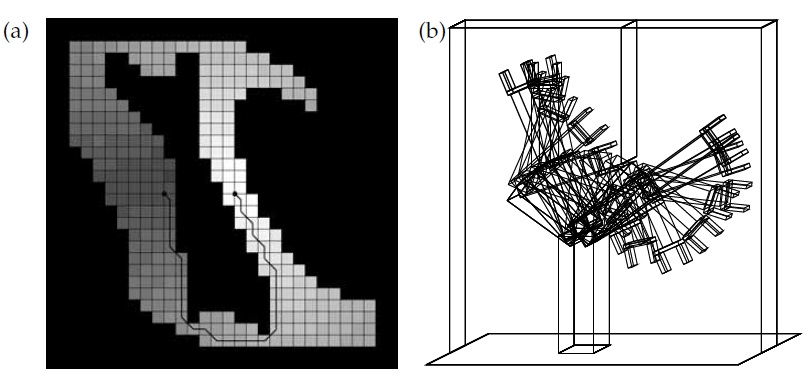
\includegraphics[width=0.9\linewidth]{147orig}}
	\caption{ ( Рис. 14.7  Итерационный алгоритм, используемая для грубой дискретизации пространства конфигураций(a).  Путь в локальных координатах рабочего пространства (b). Робот действительно избегает вертикального препятствия.) }
	\label{fig:147orig}
\end{figure}

\begin{figure}[H]
	\center{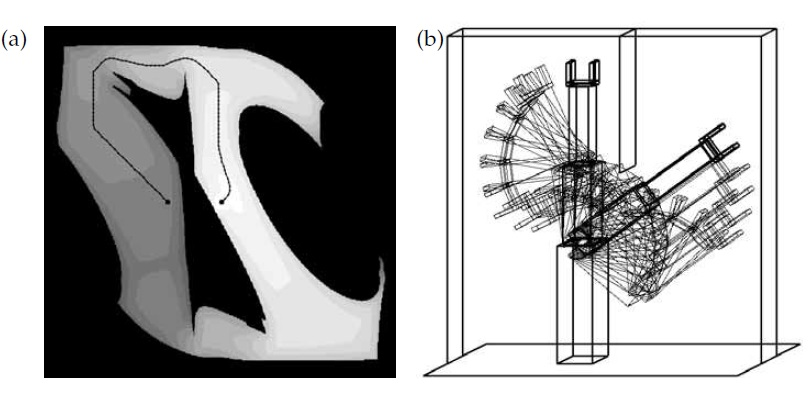
\includegraphics[width=0.9\linewidth]{148orig}}
	\caption{ ( Рис. 14.8 Вероятностный итерационный алгоритм, показан на мелкой сетке(a).  Соответствующий путь (b).) }
	\label{fig:148orig}
\end{figure}			
Второй пример приведён на Рис. 14.6a, на котором  показана модель манипулятора робота с двумя степенями свободы вращения (DOF), в плечевом и локтевом сочленениях. Обычно возможно точно определить конфигурацию этих сочленений, с помощью энкодеров на валах, соединённых с сочленениями. Поэтому, аппроксимация в (14.19) является применимой. Однако, движение манипулятора робота часто подвержено зашумлению, и эти шумы управления необходимо учитывать при планировании движения. Это делает управление манипулятором основной задачей для вероятностных алгоритмов MDP.\\

ПРОСТРАНСТВО КОНФИГУРАЦИИ\\

Движение манипулятора робота обычно описывается в \textit{пространстве конфигураций}. Пространство конфигураций для манипулятора показано на Рис. 14.6b. Здесь по горизонтальной оси показано вращательное положение плечевого сочленения, а по вертикали – ориентация в пространстве локтевого сочленения. Таким образом, каждая точка на диаграмме соответствует конкретной конфигурации. Маленькая точка на Рис. 14.6b соответствует конфигурации, показанной на Рис. 14.6a.

Принято разбивать пространство конфигураций на зоны, в которых робот может двигаться, и зоны, где может произойти столкновение. Это показано на Рис. 14.6b. Белая область на рисунке соответствует конфигурационному пространству, где столкновений не происходит, обычно называемому свободным пространством. Чёрная граница конфигурационного пространства является ограничением, накладываемым поверхностью стола и защитной клеткой. Вертикальное препятствие, проходящее в рабочее пространство робота сверху на Рис. 14.6a, соответствует светло-серому препятствию в центре Рис. 14.6b. Этот рисунок не так очевиден, и читатель может понадобиться некоторое время на визуализацию условий, при которых робот сталкивается с препятствием.

На Рис. 14.7a показан результат итерационного алгоритма на основе грубой дискретизации конфигурационного пространства. Здесь доход распространяются с помощью детерминированной модели движения, а также показан результирующий путь. Выполнение политики даёт движение, показанное на Рис. 14.7b. На Рис. 14.8 показан результат работы вероятностной модели движения, а также итоговое движение манипулятора. И снова, была применён итерационный алгоритм с допущением, что конфигурация манипулятора робота полностью наблюдаема – редкий случай, когда это действительно так!\\

\textbf{14.5	Выводы}\\

В этой главе представлен основной понятийный аппарат вероятностного управления.

•	Было определено два основных типа неопределённости, с которым может столкнуться робот: неопределённость по отношению к управлению, и неопределённость в восприятии. Первое затрудняет прогнозирование будущих событий, а второе - текущей ситуации. Неопределённость от непредсказуемых событий среды также, по умолчанию, укладывается в эту классификацию.\\

•	Цель управления была определена через \textit{функцию дохода}, проектирующая сигналы управления и состояния в виде  некоторого множества значений "желательности". Понятие "вознаграждения" позволяет выразить цели деятельности робота, а также "стоимость" такой деятельности. Общей целью управления является максимизация всех "вознаграждений", как немедленных, так и в будущие моменты времени. Чтобы избежать появления бесконечных сумм, вводится так называемый "коэффициент переоценки", экспоненциально уменьшающий будущий "доход".\\

•	Обсуждался подход к решению вероятностных проблем управления путём определения политики управления. Политика управления определяет выбор управляющего действия в виде функции информации робота об окружающем мире. Политика оптимальна, если она максимизирует сумму всех накопленных вознаграждений в будущем. Политика вычисляется на этапе планирования, который предшествует действиям робота. После вычисления она определяет оптимальные действия для любой возможной ситуации, с которой может столкнуться робот.\\

•	Был выведен конкретный алгоритм нахождения оптимальной политики управления для ограниченного случая полностью наблюдаемой среды, в которой состояние полностью наблюдаемо. Такие случаи называются марковскими процессами принятия решений. Алгоритм включает вычисление функции дохода, которая измеряет ожидаемый суммарный выигрыш. Функция дохода определяет политику путём жадного выбора управляющего действия, которое максимизирует доход. Если функция дохода оптимальна, оптимальна и политика. Итерационный алгоритм  последовательно выполняет улучшает функцию дохода с помощью рекурсивного обновления.\\

•	Были обсуждены примеры итерационного алгоритма MDP в задачах вероятностной робототехники. Для этого была извлечена мода оценки состояния, и аппроксимировано значение функции дохода с помощью сетки низкой размерности. Результатом стал алгоритм планирования движения для стохастических сред, позволивший роботу выполнять навигацию даже если эффекты действий не детерминированы.\\

Материал данной главы закладывает основу для следующей, где мы коснёмся более общей задачи управления при наличии неопределённости измерений, также известной как задача марковских процессов принятия решений с частичной наблюдаемостью. На уровне догадок уже обсуждалось, почему эта проблема намного более трудна по сравнению с MDP. В любом случае, некоторые выводы и базовые алгоритмы применимы и для более общей задачи.

Завершим эту главу упоминанием о том, что существует множество альтернативных методов вероятностного планирования и управления в условиях наличия неопределённости. Наш выбор итерации значений в качестве базового метода основан на его популярности. Кроме того, методы итерации значений являются одними из наиболее хорошо изученных для более общего случая POMDP.

Итерационный алгоритм ни в коем случае не является самым эффективным алгоритмом для генерирования сигналов управления. Известные алгоритмы планирования включают A* алгоритм, использующий эвристику при вычислении функции дохода, или методы прямого поиска политики, которые идентифицируют оптимальную локальную политику с помощью градиентного спуска. Однако, итерационный алгоритм играет ключевую роль в следующей главе, посвящённой значительно более сложному случаю оптимального управления при наличии неопределённости датчиков.\\

\textbf{14.6	Библиографические примечания}\\

Идея динамического программирования восходит к работам Беллмана (Bellman, 1957) и Говарда (Howard, 1960). Беллман (Bellman, 1957) определил уравнение равновесия для итерационного алгоритма, позже  названного его именем. Марковские процессы принятия решений (MDP) с неполной оценкой состояния впервые обсуждались Астромом (Astrom, 1965), а также Майном и Осаки (Mine and Osaki, 1970) в ранних работах по марковским процессам принятия решений. Начиная с этого момента динамическое программирование управления стало очень обширным направлением, как свидетельствует одна из недавних книг (Bertsekas and Tsitsiklis 1996). Последние улучшения базовой парадигмы включают методы итерационный алгоритм в реальном времени (Korf 1988), итерационный алгоритм, управляемый взаимодействием со средой (Barto et al. 1991), без модели (Watkins 1989), с параметрическим выражением функции ценности (Roy and Tsitsiklis 1996; Gordon 1995), или использования деревьев (Moore 1991) (также см. (Mahadevan and Kaelbling 1996)). Иерархические представления итерационного алгоритма были разработаны Парром и Расселлом (Parr and Russell, 1998) а Дитерих (Dietterich, 2000), и Бутилер (Boutilier et al., 1998) улучшили его эффективность в MDP с помощью анализа достижимости. Существует обширный набор литературы по приложению итерационного алгоритма, например, работа Барнив (Barniv, 1990) по обнаружению движущейся цели. В свете этой обширной литературы, материал в этой главе даёт лишь базовое представление самых простых методов итерационного алгоритма, позволяя подготовиться к изложению в следующей главе.

В робототехнике проблема планирования движения робота обычно исследуется без применения вероятностного подхода. Как было отмечено, подразумевается, что и состояние робота, и окружающая среда полностью известны и имеют детерминированы эффекты. Затруднения возникают из того факта, что пространство состояний непрерывно и имеет высокую размерность. Общепризнанная работа в этой области принадлежит Латомбу (Latombe, 1991). За ним следует основополагающая работа по многим базовым методам планирования движения, графам видимости (Wesley and Lozano-Perez 1979), управлению потенциальными полями (Khatib 1986), и известный алгоритм силуэтов Канни (Canny, 1987). Роват (Rowat, 1979) представил идею графов Вороного в области управления роботом, а Гуйбас (Guibas et al., 1992) показал способ их эффективного вычисления. Чозет (Choset, 1996) развил эту парадигму в семейство эффективных алгоритмов исследования и картографии. Другой набор методов использует рандомизированный (но не вероятностный!) подход к поиску в пространстве возможных путей робота (Kavraki and Latombe 1994). Актуальная книга по этому вопросу была написана Чозетом (Choset et al., 2004).

АППРОКСИМАЦИЯ РАЗБИЕНИЯ НА ЯЧЕЙКИ\\

В области планирования движения робота в этой главе обсуждались методы \textit{аппроксимации разбиения на ячейки},  которые, в детерминированном случае, не гарантируют полноту. 
Разбиения непрерывных пространств на конечные графы изучалось в робототехнике десятилетиями. Рейф (Reif, 1979) разработал множество методов разбиения непрерывных пространств на конечное множество ячеек, сохраняющих полноту в планировании движения. Идея пространств конфигураций Необходимых для проверки пересечений с другими методами в этой главе, была изначально предложена Лозано-Перезом (Lozano-Perez, 1983). Методы рекурсивного разбиения ячеек для планирования конфигурационного пространства можно найти в работах Брукса и Лозано-Переза (Brooks and Lozano-Perez, 1985), но для идеальных допущений об идеальных моделях среды и роботов. Действия при частичной осведомлённости были описаны Голдбергом (Goldberg, 1993), в кандидатской диссертации которого были разработаны алгоритмы для частичного ориентирования в отсутствии датчиков. Шарма (Sharma, 1992) разработал методы планирования пути робота со стохастическими препятствиями.

Функции политики, назначающие управляющее действие для каждого возможного состояния робота известны как \textit{контроллеры}. Алгоритм вывода политики управления часто называют \textit{оптимальным контроллером} (Bryson and Yu-Chi 1975). Политики управления также называют \textit{навигационной функцией} (Koditschek 1987; Rimon and Koditschek 1992). В области искусственного интеллекта они известны как универсальные пути (Schoppers 1987), и многие алгоритмы символического планирования касаются проблемы нахождения таких универсальных планов (Dean et al. 1995; Kushmerick et al. 1995; Hoey et al. 1999). Некоторые работы в робототехнике были посвящены соединению универсальных планов и последовательностей действий с открытой петлей, например, в кандидатской диссертации Нурбахша (Nourbakhsh, 1987).

Также заметим, что запись «управления» в книге употребляется в несколько узком смысле. В главе специально не описаны стандартные методы в широкой области управления, такие, как управление PID и другие популярные методы, которые легко найти в учебниках (Dorf and Bishop 2001). Очевидно, такие методы необходимы и применимы во многих робототехнических системах для реального мира. Сознательный отказ от описания таких методов основан не на ограничениях объёма, и на том, что эти методы не полагаются на явное выражение неопределённости.\\

\textbf{14.7	Упражнения}\\

1.	Алгоритм динамического программирования использует наиболее вероятное состояние для определения действия. Изобразить среду робота, в которой зависимость действий от наиболее вероятного состояния является неверным выбором? Можно ли указать конкретные причины, почему такой выбор может быть неверным?\\

2.	Допустим, итерационный алгоритм для фиксированной функции дохода выполняется до окончания. Затем функция дохода меняется. Требуется изменить функцию дохода в дальнейших итерациях алгоритма, используя предыдущую функцию как начальную точку.\\

(a)	Является ли это хорошим или плохим выбором? Зависит ли ответ от увеличения или уменьшения дохода?\\

(b)	Можно ли, навскидку, сформулировать алгоритм, который будет более эффективным, чем просто продолжение итерационного алгоритма после изменения дохода? Если возможно, указать причины большей эффективности предложенного алгоритма. Если нет, указать причину, почему такой алгоритм существовать не может.\\

3.	"Рай или Ад"? В этом упражнении требуется выполнить обобщение динамического программирования к среде с единственной переменной со скрытым состоянием. Среда представляет собой лабиринт с определенным стартом, обозначенным «S» и два возможных целевых состояния, отмеченных «H»

\begin{figure}[H]
	\center{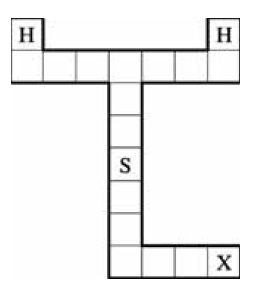
\includegraphics[width=0.3\linewidth]{laborig}}
	\label{fig:laborig}
\end{figure}

Агент не знает, какое из двух целевых состояний даст положительную награду. Одно состояние даст +100, а другое -100. Существует вероятность 0,5 что каждое из этих состояний истинно.  Стоимость перемещения -1, агент может перемещаться только в четырёх направлениях -  север, юг, запад, восток. Как только достигнуто состояние “H”, игра окончена.\\

(a)	Реализовать итерационный алгоритм для этого сценария (игнорируя метку “X” на рисунке). Вычисляет ли предложенная реализация значение стартового состояния? Какова оптимальная политика?\\

(b)	Изменить итерационный алгоритм для обработки вероятностной модели измерений: с вероятностью 0,9 агент двигается в указанном направлении, с вероятностью 0,1 – случайным образом перемещается по одному из трёх других направлений. Снова запустить итерационный алгоритм, вычислить значение в стартовом состоянии и оптимальную политику.\\

(c)	Допустим, что в местоположении “X” стоит знак, информирующий агента о том, какая награда находится в каждом из состояний, обозначенных “H.” Как это повлияет на оптимальную политику?\\

(d)	Как можно изменить итерационный алгоритм для нахождения оптимальной политики? Указать конкретные шаги. Указать изменения пространства, по которому изменяется значение дохода.\\

(e)	Реализовать модификацию, вычислить значение в стартовом состоянии и оптимальную политику.\\



 
\end{document}